\documentclass{ximera}

\title{This is the sample!}
\author{A Ximera Author}

\begin{abstract}
  This is a place to get started.
\end{abstract}

\begin{document}
\maketitle

Here's a circle.

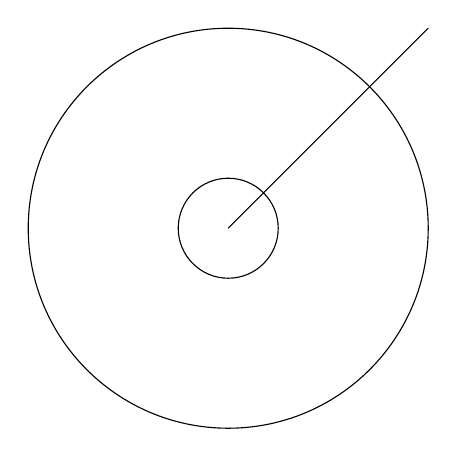
\begin{tikzpicture}
  \draw (0,0) circle (1in);
  \draw (0,0) circle (0.25in);
  \draw (0,0) -- (1in,1in);
\end{tikzpicture}

\begin{problem}
\begin{multipleChoice}
\choice{Incorrect}
\choice{Not this one!}
\choice[correct]{Click here?}
\choice{Not me!}
\end{multipleChoice}
\end{problem}

\begin{problem}
   You can test that $x + x = \answer{2x}$ or that $x \cdot x = \answer{x^2}$.
\end{problem}

\begin{problem}
   The tolerance 0.01 means $\pi \approx \answer[tolerance=0.01]{3.141592653}$
\end{problem}

\begin{problem}
   The tolerance 17 means $3421 \approx \answer[tolerance=17]{3421}$
\end{problem}

\end{document}
